
\chapter{Minimum-Weight Perfect Matching decoder}\label{ch:mwpm}

In this chapter, we will give a short description of the most commonly used decoder for surface codes: the Minimum-Weight Perfect Matching decoder. This decoder was actually the first decoder for surface code, first introduced in \cite{dennis2002topological}. The Minimum-Weight Perfect Matching decoder has a worst-case complexity of between $\m{O}(n^3)$ and $\m{O}(n^7)$, depending on the implementation \cite{edmonds1965paths, kolmogorov2009blossom}, but has a relatively high decoder threshold. Many have improved upon the decoder to extend it to more general noise models or to optimize its performance \cite{fowler2012towards, fowler2012surface, fowler2013optimal, stace2009thresholds, stace2010error}. Most notably, at the cost of space complexity, the average-case complexity of the decoder has been reduced to $\m{O}(1)$ time \cite{fowler2013minimum}. We will outline the idea of the Minimum-Weight Perfect Matching decoder in Section \ref{sec:mwpm} and show its performance on a simulated lattice in Section \ref{sec:mwpmperformance}.

\section{Minimum-weight perfect matching}\label{sec:mwpm}

Recall from Section \ref{sec:quasiparticle} that decoding a surface code can be simply performed by pairing anyons in the syndrome. The challenge for the decoder is choosing a pairing that is not likely to result in a logical error. 

The basic principle behind the minimum-weight perfect matching approach is to identify the \emph{lowest weight} error configuration that can produce the observed syndrome $\sigma$. If independent errors occur on a lattice of $N$ qubits with probability $p$, then the probability of some error operator $\hat{E}$ with $|\hat{E}|$ errors has a probability of occurring
\begin{equation}
  P(\hat{E}) = p^{\abs{\hat{E}}}(1-p)^{N-\abs{\hat{E}}},
\end{equation}
and therefore
\begin{equation}
  P(\hat{E})\propto \left(\frac{p}{1-p}\right)^\abs{\hat{E}}.
\end{equation}
As $0<p/(1-p)<1$, the probability of $\hat{E}$ occurring is maximized when $|\hat{E}|$ is minimized. This means that the error configuration with the smallest amount of errors is the most probable one. 

Recall from Section \ref{sec:correction} that to correct an error, the goal is to find the correction operator $\hat{C}$ that is most likely to return the code to the codespace. Finding the lowest weight configuration does not correspond to this problem. To find the correction that is most likely, one would have to consider \emph{all} possible error configuration that could produce the observed syndrome $\sigma$, find to which class they belong and weigh each class accordingly to find the most likely correction. The lowest weight configuration is in general a good approximation of the decoding problem, but not in all cases. It is due to this discrepancy that the error threshold of the Minimum-Weight Perfect Matching decoder is lower than the optimal value. 

For a set of anyons in the quasiparticle representation, finding the minimum-weighted pairs is equivalent to finding the minimal distances between the particles. The distance between two anyons is the shortest path between them, where a path consists of a number of qubits that is equal to the weight. This problem can be efficiently solved by mapping the quasiparticles into a graph matching problem, where every anyon is a node in a completely connected graph. The edges in the graph are now assigned a weight corresponding to the distance between the anyons (Figure \ref{fig:mwpm}). This graphing problem can now be solved in polynomial time using Edmonds' blossom algorithm \cite{edmonds1965paths}. 

\tikzstyle{rednode}=[circle, fill=red!50, minimum size=1.5]
\tikzstyle{line}=[line width=1]
\tikzstyle{node}=[midway, font=\footnotesize]
\newcommand{\drawmwpmgrid}{
  \draw[step=.4cm, opacity=.25] (-.4,-.4) grid (4.4,4.4);
  \draw (-.4,-.4) rectangle (4.4,4.4);
  \node[rednode] (1) at (0.5,0.4)  {};
  \node[rednode] (2) at (2,0.7)    {};
  \node[rednode] (3) at (2.5,1.2)  {};
  \node[rednode] (4) at (4,1)      {};
  \node[rednode] (5) at (0.75,2.1) {};
  \node[rednode] (6) at (1.95,2.4) {};
  \node[rednode] (7) at (1.6, 3.4) {};
  \node[rednode] (8) at (2.7, 3.5) {};
}
\begin{figure}[htbp]
    \centering
    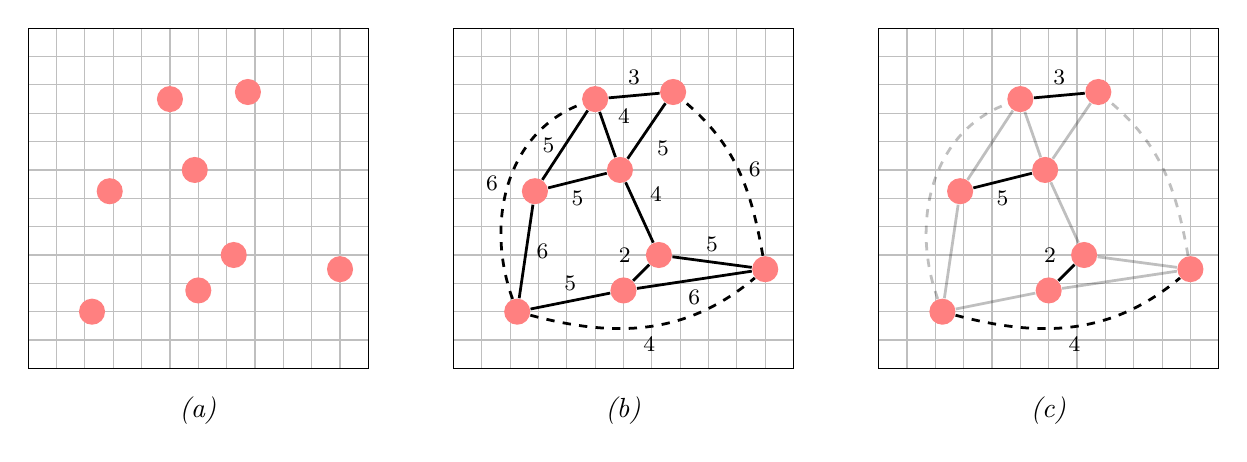
\begin{tikzpicture}[scale=0.9]
      \drawmwpmgrid
      \node at (2,-1) {\emph{(a)}};
    
      \begin{scope}[shift={(6,0)}]
        \drawmwpmgrid
        \draw[line] (2) -- (1) node[node,above]{5} -- (5) node[node, right]{6} -- (6) node[node, below]{5} -- (7) node[node, above right]{4} -- (8) node[node, above]{3} -- (6) node[node, below right]{5};
        \draw[line] (2) -- (3) node[node, above left]{2} -- (4) node[node, above]{5} -- (2) node[node, below]{6};
        \draw[line] (6) -- (3) node[node,above right]{4};
        \draw[line] (5) -- (7) node[node, left]{5};
        \draw[line, dashed] (1) to [out=-15, in=220] node[node,below]{4} (4);
        \draw[line, dashed] (4) to [out=100, in=-40] node[node,right]{6} (8);
        \draw[line, dashed] (1) to [out=110, in=200] node[node,left]{6} (7);
        \node at (2,-1) {\emph{(b)}};

      \end{scope}
      
      \begin{scope}[shift={(12,0)}]
        \drawmwpmgrid
        \draw[line, opacity=.25] (6) -- (3) -- (4) -- (2) -- (1);
        \draw[line, opacity=.25] (1) -- (5) -- (7) -- (6) -- (8) ;
        \draw[line] (7) -- (8) node[node, above]{3};
        \draw[line] (5) -- (6) node[node, below]{5};
        \draw[line] (2) -- (3) node[node, above left]{2};
        \draw[line, dashed] (1) to [out=-15, in=220] node[node,below]{4} (4);
        \draw[line, dashed, opacity=.25] (4) to [out=100, in=-40] (8);
        \draw[line, dashed, opacity=.25] (1) to [out=110, in=200] (7);
        \node at (2,-1) {\emph{(c)}};

      \end{scope}
    \end{tikzpicture}
    \caption{Visualizing the graph matching problem of minimum-weight pairs between anyons. (a) The set of anyons from the measured syndrome are the nodes in the graph matching problem. (b) The graph is initiated by connecting all nodes in the graph with edges weighted correspondingly to the shortest distance between the anyons. High weight edges have been excluded here for clarity. (c) The minimum-weight subset of edges is the result. This figure is inspired by others \cite{naomi2016thesis}.}\label{fig:mwpm}
  \end{figure}
  

\section{Boundaries}\label{sec:mwpmboundaries}

For surfaces with boundaries such as the planar code (Section \ref{sec:surface_planar}), the number of anyons in the syndrome is now not guaranteed to be even. In the graph representation, an error on an edge in $\m{E}_delta$ will cause only a non-trivial syndrome measurement on one of its supporting vertices. The other vertex is in the open vertex set $\m{V}_\omega$, which are not equivalent to ancilla qubits or stabilizer measurements. Thus, the concept of pairing must include the possibility of an anyon to pair with the code boundary, in addition to paring with other anyons. 

The procedure of mapping anyons to a graph matching problem must now be modified to include this extra pairing possibility. This is done by creating for every anyon an extra ``virtual'' node in the graph that is located at the boundary of the code as described by \cite{wang2011surface}. The node corresponding to the anyon is connected by an edge with its virtual pair. Furthermore, the set of virtual nodes are all connected by edges of weight 0. This allows a node to pair with the virtual node at the boundary, and all ``unused'' virtual nodes to pair with each other such that they are efficiently removed. 

\section{Performance}\label{sec:mwpmperformance}

We benchmark the performance of the Minimum-Weight Perfect Matching decoder using our own implementation in Python3 (see Appendix \ref{ap:oopsurfacecode}) for a simulated lattice and the BlossomV algorithm, which is implemented in C, for finding the minimum-weight matching \cite{kolmogorov2009blossom}. This is done by Monte Carlo simulations of decoding on a simulated lattice and to fit for the code threshold as described in Section \ref{sec:simthres}. For the independent noise model (Definition \ref{def:independent}), we simulate on lattice sizes $[8, 16, 24, 32, 40, 48, 56, 64]$ with a minimum of $52.800$ samples. For the phenomenological noise model (Definition \ref{def:pheno}), we simulate on lattice sizes $L_{small}=[8,10,12,14,16,18,20,22]$ with a minimum of $52.800$ samples. The code thresholds for the toric and planar codes with independent and phenomenological noise are listed in Table \ref{tab:mwpm}.

\begin{table}[htpb]
  \centering
  \begin{tabularx}{\textwidth} { | R{1} || C{1.5} | C{.5} | C{1.5} | C{.5} | }
   \hline
   & \multicolumn{2}{c|}{Independent noise}& \multicolumn{2}{c|}{Phenomenal noise} \\
   \hline
   & $p_{th}$ & $k_C$ & $p_{th}$ & $k_C$ \\
   \hhline{|=#=|=|=|=|}
   Toric code & $0.10349 \pm 0.00004$ & $0.7158$ & $0.02965 \pm 0.00003$ & $0.9024$ \\
   \hline
   Planar code  & $0.10292 \pm 0.00005$ & $0.8478$ & $0.02928 \pm 0.00003$ & $0.928$ \\
  \hline
  \end{tabularx}
  \caption{Error thresholds for the Minimum-Weight Perfect Matching decoder utilizing the BlossomV algorithm \cite{kolmogorov2009blossom} on both the toric and planar lattices with independent and phenomenological noise. The results of the Monte Carlo simulations used to calculate the thresholds are included in Figure \ref{fig:threshold_mwpm}.}\label{tab:mwpm}
\end{table}

These obtained values for the decoder threshold $p_{th}$ correspond with the values reported in the literature \cite{dennis2002topological, naomi2016thesis, wang2009threshold, wang2003confinement}. In de Monte Carlo simulations, some metadata are also acquired that will be useful when comparing the performance of the Minimum-Weight Perfect Matching decoder with other decoders. Most notably, the average running time of the simulation and the actual weight of the matching are used as metrics in the upcoming chapters. 